\documentclass{standalone}
\usepackage{tikz}
\usetikzlibrary{patterns, positioning}


\begin{document}
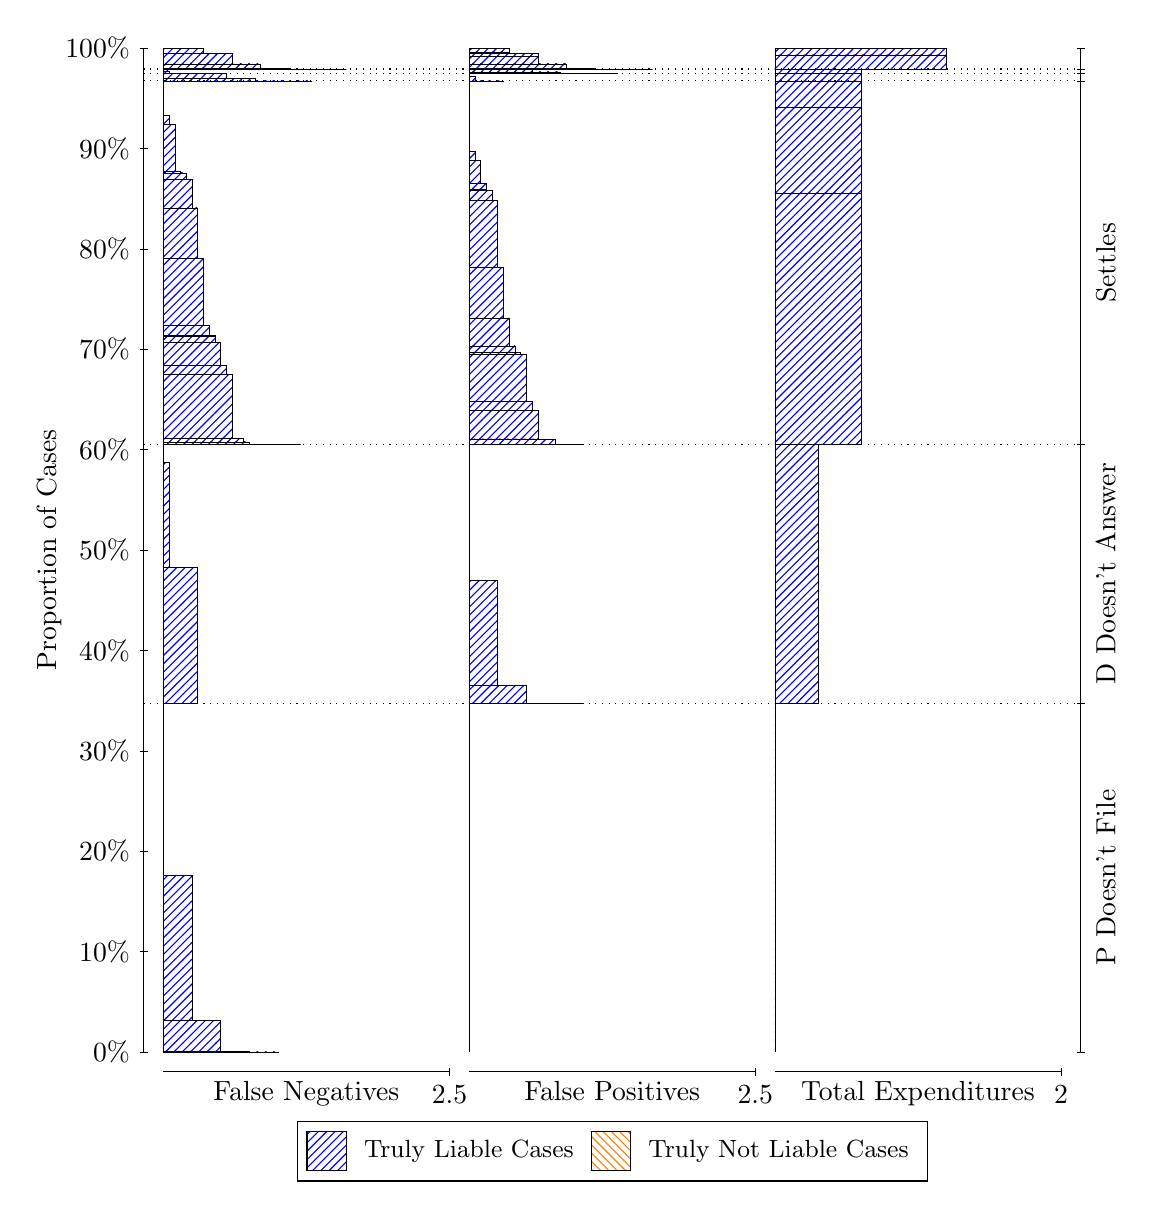
\begin{tikzpicture}
\draw[black, very thin] (1.5,1.75) -- (1.5,14.5);
\node[rotate=90, text=black, anchor=center] at (0.3, 8.125) {Proportion of Cases};
\draw[black, very thin] (1.45,1.75) -- (1.55,1.75);
\node[text=black, anchor=east] at (1.45, 1.75) {0\%};
\draw[black, very thin] (1.45,3.025) -- (1.55,3.025);
\node[text=black, anchor=east] at (1.45, 3.025) {10\%};
\draw[black, very thin] (1.45,4.3) -- (1.55,4.3);
\node[text=black, anchor=east] at (1.45, 4.3) {20\%};
\draw[black, very thin] (1.45,5.575) -- (1.55,5.575);
\node[text=black, anchor=east] at (1.45, 5.575) {30\%};
\draw[black, very thin] (1.45,6.85) -- (1.55,6.85);
\node[text=black, anchor=east] at (1.45, 6.85) {40\%};
\draw[black, very thin] (1.45,8.125) -- (1.55,8.125);
\node[text=black, anchor=east] at (1.45, 8.125) {50\%};
\draw[black, very thin] (1.45,9.4) -- (1.55,9.4);
\node[text=black, anchor=east] at (1.45, 9.4) {60\%};
\draw[black, very thin] (1.45,10.675) -- (1.55,10.675);
\node[text=black, anchor=east] at (1.45, 10.675) {70\%};
\draw[black, very thin] (1.45,11.95) -- (1.55,11.95);
\node[text=black, anchor=east] at (1.45, 11.95) {80\%};
\draw[black, very thin] (1.45,13.225) -- (1.55,13.225);
\node[text=black, anchor=east] at (1.45, 13.225) {90\%};
\draw[black, very thin] (1.45,14.5) -- (1.55,14.5);
\node[text=black, anchor=east] at (1.45, 14.5) {100\%};

\draw[black, very thin] (13.4,1.75) -- (13.4,14.5);
\draw[black, very thin] (13.35,1.75) -- (13.45,1.75);
\node[anchor=west] at (13.35, 1.75) {};
\draw[black, very thin] (13.35,6.1798) -- (13.45,6.1798);
\node[anchor=west] at (13.35, 6.1798) {};
\draw[black, very thin] (13.35,9.462) -- (13.45,9.462);
\node[anchor=west] at (13.35, 9.462) {};
\draw[black, very thin] (13.35,14.082) -- (13.45,14.082);
\node[anchor=west] at (13.35, 14.082) {};
\draw[black, very thin] (13.35,14.175) -- (13.45,14.175);
\node[anchor=west] at (13.35, 14.175) {};
\draw[black, very thin] (13.35,14.233) -- (13.45,14.233);
\node[anchor=west] at (13.35, 14.233) {};
\draw[black, very thin] (13.35,14.5) -- (13.45,14.5);
\node[anchor=west] at (13.35, 14.5) {};

\draw[black, very thin, pattern color=blue, pattern=north east lines] (1.75,1.75) rectangle (3.2033,1.7501);
\draw[black, very thin, pattern color=blue, pattern=north east lines] (1.75,1.7501) rectangle (2.84,1.7624);
\draw[black, very thin, pattern color=blue, pattern=north east lines] (1.75,1.7624) rectangle (2.4767,2.1497);
\draw[black, very thin, pattern color=blue, pattern=north east lines] (1.75,2.1497) rectangle (2.1133,3.9975);
\draw[black, very thin, pattern color=orange, pattern=north west lines] (1.75,3.9975) rectangle (1.75,3.9975);
\draw[black, very thin, pattern color=blue, pattern=north east lines] (1.75,3.9975) rectangle (1.75,6.1798);
\draw[black, very thin, pattern color=blue, pattern=north east lines] (1.75,6.1798) rectangle (2.186,7.9039);
\draw[black, very thin, pattern color=blue, pattern=north east lines] (1.75,7.9039) rectangle (1.8227,9.241);
\draw[black, very thin, pattern color=orange, pattern=north west lines] (1.75,9.241) rectangle (1.75,9.241);
\draw[black, very thin, pattern color=blue, pattern=north east lines] (1.75,9.241) rectangle (1.75,9.462);
\draw[black, very thin, pattern color=blue, pattern=north east lines] (1.75,9.462) rectangle (3.494,9.462);
\draw[black, very thin, pattern color=blue, pattern=north east lines] (1.75,9.462) rectangle (3.2033,9.4621);
\draw[black, very thin, pattern color=blue, pattern=north east lines] (1.75,9.4621) rectangle (3.1307,9.4632);
\draw[black, very thin, pattern color=blue, pattern=north east lines] (1.75,9.4632) rectangle (3.058,9.4632);
\draw[black, very thin, pattern color=blue, pattern=north east lines] (1.75,9.4632) rectangle (2.9127,9.4636);
\draw[black, very thin, pattern color=blue, pattern=north east lines] (1.75,9.4636) rectangle (2.84,9.4988);
\draw[black, very thin, pattern color=blue, pattern=north east lines] (1.75,9.4988) rectangle (2.7673,9.5412);
\draw[black, very thin, pattern color=blue, pattern=north east lines] (1.75,9.5412) rectangle (2.6947,9.5473);
\draw[black, very thin, pattern color=blue, pattern=north east lines] (1.75,9.5473) rectangle (2.622,10.355);
\draw[black, very thin, pattern color=blue, pattern=north east lines] (1.75,10.355) rectangle (2.5493,10.473);
\draw[black, very thin, pattern color=blue, pattern=north east lines] (1.75,10.473) rectangle (2.4767,10.761);
\draw[black, very thin, pattern color=blue, pattern=north east lines] (1.75,10.761) rectangle (2.404,10.842);
\draw[black, very thin, pattern color=blue, pattern=north east lines] (1.75,10.842) rectangle (2.404,10.851);
\draw[black, very thin, pattern color=blue, pattern=north east lines] (1.75,10.851) rectangle (2.3313,10.978);
\draw[black, very thin, pattern color=blue, pattern=north east lines] (1.75,10.978) rectangle (2.2587,11.833);
\draw[black, very thin, pattern color=blue, pattern=north east lines] (1.75,11.833) rectangle (2.186,12.471);
\draw[black, very thin, pattern color=blue, pattern=north east lines] (1.75,12.471) rectangle (2.1133,12.828);
\draw[black, very thin, pattern color=blue, pattern=north east lines] (1.75,12.828) rectangle (2.0407,12.913);
\draw[black, very thin, pattern color=blue, pattern=north east lines] (1.75,12.913) rectangle (2.0407,12.913);
\draw[black, very thin, pattern color=blue, pattern=north east lines] (1.75,12.913) rectangle (1.968,12.935);
\draw[black, very thin, pattern color=blue, pattern=north east lines] (1.75,12.935) rectangle (1.8953,13.534);
\draw[black, very thin, pattern color=blue, pattern=north east lines] (1.75,13.534) rectangle (1.8227,13.644);
\draw[black, very thin, pattern color=orange, pattern=north west lines] (1.75,13.644) rectangle (1.75,13.644);
\draw[black, very thin, pattern color=blue, pattern=north east lines] (1.75,13.644) rectangle (1.75,14.082);
\draw[black, very thin, pattern color=blue, pattern=north east lines] (1.75,14.082) rectangle (3.6393,14.082);
\draw[black, very thin, pattern color=blue, pattern=north east lines] (1.75,14.082) rectangle (3.276,14.082);
\draw[black, very thin, pattern color=blue, pattern=north east lines] (1.75,14.082) rectangle (2.9127,14.117);
\draw[black, very thin, pattern color=blue, pattern=north east lines] (1.75,14.117) rectangle (2.5493,14.174);
\draw[black, very thin, pattern color=blue, pattern=north east lines] (1.75,14.174) rectangle (2.186,14.175);
\draw[black, very thin, pattern color=orange, pattern=north west lines] (1.75,14.175) rectangle (1.75,14.175);
\draw[black, very thin, pattern color=blue, pattern=north east lines] (1.75,14.175) rectangle (2.186,14.176);
\draw[black, very thin, pattern color=blue, pattern=north east lines] (1.75,14.176) rectangle (1.8227,14.211);
\draw[black, very thin, pattern color=orange, pattern=north west lines] (1.75,14.211) rectangle (1.75,14.211);
\draw[black, very thin, pattern color=blue, pattern=north east lines] (1.75,14.211) rectangle (1.75,14.233);
\draw[black, very thin, pattern color=blue, pattern=north east lines] (1.75,14.233) rectangle (4.0753,14.233);
\draw[black, very thin, pattern color=blue, pattern=north east lines] (1.75,14.233) rectangle (3.712,14.233);
\draw[black, very thin, pattern color=blue, pattern=north east lines] (1.75,14.233) rectangle (3.3487,14.237);
\draw[black, very thin, pattern color=blue, pattern=north east lines] (1.75,14.237) rectangle (2.9853,14.299);
\draw[black, very thin, pattern color=blue, pattern=north east lines] (1.75,14.299) rectangle (2.622,14.434);
\draw[black, very thin, pattern color=blue, pattern=north east lines] (1.75,14.434) rectangle (2.2587,14.495);
\draw[black, very thin, pattern color=blue, pattern=north east lines] (1.75,14.495) rectangle (1.8953,14.5);
\draw[black, very thin, pattern color=orange, pattern=north west lines] (1.75,14.5) rectangle (1.75,14.5);
\draw[black, very thin, pattern color=blue, pattern=north east lines] (1.75,14.5) rectangle (1.75,14.5);
\draw[black, very thin, pattern color=orange, pattern=north west lines] (5.6333,1.75) rectangle (5.6333,1.75);
\draw[black, very thin, pattern color=blue, pattern=north east lines] (5.6333,1.75) rectangle (5.6333,6.1798);
\draw[black, very thin, pattern color=orange, pattern=north west lines] (5.6333,6.1798) rectangle (7.0867,6.1798);
\draw[black, very thin, pattern color=blue, pattern=north east lines] (5.6333,6.1798) rectangle (7.0867,6.1798);
\draw[black, very thin, pattern color=blue, pattern=north east lines] (5.6333,6.1798) rectangle (6.7233,6.1809);
\draw[black, very thin, pattern color=blue, pattern=north east lines] (5.6333,6.1809) rectangle (6.36,6.4009);
\draw[black, very thin, pattern color=blue, pattern=north east lines] (5.6333,6.4009) rectangle (5.9967,7.738);
\draw[black, very thin, pattern color=blue, pattern=north east lines] (5.6333,7.738) rectangle (5.6333,9.462);
\draw[black, very thin, pattern color=orange, pattern=north west lines] (5.6333,9.462) rectangle (7.0867,9.462);
\draw[black, very thin, pattern color=blue, pattern=north east lines] (5.6333,9.462) rectangle (7.0867,9.4622);
\draw[black, very thin, pattern color=orange, pattern=north west lines] (5.6333,9.4622) rectangle (6.9413,9.4622);
\draw[black, very thin, pattern color=blue, pattern=north east lines] (5.6333,9.4622) rectangle (6.9413,9.4622);
\draw[black, very thin, pattern color=orange, pattern=north west lines] (5.6333,9.4622) rectangle (6.796,9.4622);
\draw[black, very thin, pattern color=blue, pattern=north east lines] (5.6333,9.4622) rectangle (6.796,9.4626);
\draw[black, very thin, pattern color=blue, pattern=north east lines] (5.6333,9.4626) rectangle (6.7233,9.5331);
\draw[black, very thin, pattern color=orange, pattern=north west lines] (5.6333,9.5331) rectangle (6.6507,9.5331);
\draw[black, very thin, pattern color=blue, pattern=north east lines] (5.6333,9.5331) rectangle (6.6507,9.5333);
\draw[black, very thin, pattern color=blue, pattern=north east lines] (5.6333,9.5333) rectangle (6.578,9.5363);
\draw[black, very thin, pattern color=orange, pattern=north west lines] (5.6333,9.5363) rectangle (6.5053,9.5363);
\draw[black, very thin, pattern color=blue, pattern=north east lines] (5.6333,9.5363) rectangle (6.5053,9.9003);
\draw[black, very thin, pattern color=blue, pattern=north east lines] (5.6333,9.9003) rectangle (6.4327,10.01);
\draw[black, very thin, pattern color=blue, pattern=north east lines] (5.6333,10.01) rectangle (6.36,10.609);
\draw[black, very thin, pattern color=blue, pattern=north east lines] (5.6333,10.609) rectangle (6.2873,10.631);
\draw[black, very thin, pattern color=orange, pattern=north west lines] (5.6333,10.631) rectangle (6.2147,10.631);
\draw[black, very thin, pattern color=blue, pattern=north east lines] (5.6333,10.631) rectangle (6.2147,10.632);
\draw[black, very thin, pattern color=blue, pattern=north east lines] (5.6333,10.632) rectangle (6.2147,10.716);
\draw[black, very thin, pattern color=blue, pattern=north east lines] (5.6333,10.716) rectangle (6.142,11.074);
\draw[black, very thin, pattern color=blue, pattern=north east lines] (5.6333,11.074) rectangle (6.0693,11.711);
\draw[black, very thin, pattern color=blue, pattern=north east lines] (5.6333,11.711) rectangle (5.9967,12.566);
\draw[black, very thin, pattern color=blue, pattern=north east lines] (5.6333,12.566) rectangle (5.924,12.693);
\draw[black, very thin, pattern color=blue, pattern=north east lines] (5.6333,12.693) rectangle (5.8513,12.702);
\draw[black, very thin, pattern color=blue, pattern=north east lines] (5.6333,12.702) rectangle (5.8513,12.783);
\draw[black, very thin, pattern color=blue, pattern=north east lines] (5.6333,12.783) rectangle (5.7787,13.071);
\draw[black, very thin, pattern color=blue, pattern=north east lines] (5.6333,13.071) rectangle (5.706,13.189);
\draw[black, very thin, pattern color=blue, pattern=north east lines] (5.6333,13.189) rectangle (5.6333,14.082);
\draw[black, very thin, pattern color=orange, pattern=north west lines] (5.6333,14.082) rectangle (6.0693,14.082);
\draw[black, very thin, pattern color=blue, pattern=north east lines] (5.6333,14.082) rectangle (6.0693,14.083);
\draw[black, very thin, pattern color=blue, pattern=north east lines] (5.6333,14.083) rectangle (5.706,14.14);
\draw[black, very thin, pattern color=blue, pattern=north east lines] (5.6333,14.14) rectangle (5.6333,14.175);
\draw[black, very thin, pattern color=orange, pattern=north west lines] (5.6333,14.175) rectangle (7.5227,14.175);
\draw[black, very thin, pattern color=blue, pattern=north east lines] (5.6333,14.175) rectangle (7.5227,14.175);
\draw[black, very thin, pattern color=blue, pattern=north east lines] (5.6333,14.175) rectangle (7.1593,14.175);
\draw[black, very thin, pattern color=blue, pattern=north east lines] (5.6333,14.175) rectangle (6.796,14.197);
\draw[black, very thin, pattern color=blue, pattern=north east lines] (5.6333,14.197) rectangle (6.4327,14.232);
\draw[black, very thin, pattern color=blue, pattern=north east lines] (5.6333,14.232) rectangle (6.0693,14.233);
\draw[black, very thin, pattern color=orange, pattern=north west lines] (5.6333,14.233) rectangle (7.9587,14.233);
\draw[black, very thin, pattern color=blue, pattern=north east lines] (5.6333,14.233) rectangle (7.9587,14.233);
\draw[black, very thin, pattern color=orange, pattern=north west lines] (5.6333,14.233) rectangle (7.5953,14.233);
\draw[black, very thin, pattern color=blue, pattern=north east lines] (5.6333,14.233) rectangle (7.5953,14.233);
\draw[black, very thin, pattern color=orange, pattern=north west lines] (5.6333,14.233) rectangle (7.232,14.233);
\draw[black, very thin, pattern color=blue, pattern=north east lines] (5.6333,14.233) rectangle (7.232,14.238);
\draw[black, very thin, pattern color=blue, pattern=north east lines] (5.6333,14.238) rectangle (6.8687,14.299);
\draw[black, very thin, pattern color=orange, pattern=north west lines] (5.6333,14.299) rectangle (6.8687,14.299);
\draw[black, very thin, pattern color=blue, pattern=north east lines] (5.6333,14.299) rectangle (6.8687,14.299);
\draw[black, very thin, pattern color=blue, pattern=north east lines] (5.6333,14.299) rectangle (6.5053,14.396);
\draw[black, very thin, pattern color=orange, pattern=north west lines] (5.6333,14.396) rectangle (6.5053,14.396);
\draw[black, very thin, pattern color=blue, pattern=north east lines] (5.6333,14.396) rectangle (6.5053,14.434);
\draw[black, very thin, pattern color=blue, pattern=north east lines] (5.6333,14.434) rectangle (6.142,14.45);
\draw[black, very thin, pattern color=blue, pattern=north east lines] (5.6333,14.45) rectangle (6.142,14.496);
\draw[black, very thin, pattern color=blue, pattern=north east lines] (5.6333,14.496) rectangle (5.7787,14.496);
\draw[black, very thin, pattern color=blue, pattern=north east lines] (5.6333,14.496) rectangle (5.7787,14.5);
\draw[black, very thin, pattern color=blue, pattern=north east lines] (5.6333,14.5) rectangle (5.6333,14.5);
\draw[black, very thin, pattern color=orange, pattern=north west lines] (9.5167,1.75) rectangle (9.5167,1.75);
\draw[black, very thin, pattern color=blue, pattern=north east lines] (9.5167,1.75) rectangle (9.5167,6.1798);
\draw[black, very thin, pattern color=orange, pattern=north west lines] (9.5167,6.1798) rectangle (10.062,6.1798);
\draw[black, very thin, pattern color=blue, pattern=north east lines] (9.5167,6.1798) rectangle (10.062,9.462);
\draw[black, very thin, pattern color=orange, pattern=north west lines] (9.5167,9.462) rectangle (10.607,9.462);
\draw[black, very thin, pattern color=blue, pattern=north east lines] (9.5167,9.462) rectangle (10.607,12.661);
\draw[black, very thin, pattern color=orange, pattern=north west lines] (9.5167,12.661) rectangle (10.607,12.661);
\draw[black, very thin, pattern color=blue, pattern=north east lines] (9.5167,12.661) rectangle (10.607,13.743);
\draw[black, very thin, pattern color=orange, pattern=north west lines] (9.5167,13.743) rectangle (10.607,13.743);
\draw[black, very thin, pattern color=blue, pattern=north east lines] (9.5167,13.743) rectangle (10.607,14.082);
\draw[black, very thin, pattern color=orange, pattern=north west lines] (9.5167,14.082) rectangle (10.607,14.082);
\draw[black, very thin, pattern color=blue, pattern=north east lines] (9.5167,14.082) rectangle (10.607,14.175);
\draw[black, very thin, pattern color=orange, pattern=north west lines] (9.5167,14.175) rectangle (10.607,14.175);
\draw[black, very thin, pattern color=blue, pattern=north east lines] (9.5167,14.175) rectangle (10.607,14.233);
\draw[black, very thin, pattern color=orange, pattern=north west lines] (9.5167,14.233) rectangle (11.697,14.233);
\draw[black, very thin, pattern color=blue, pattern=north east lines] (9.5167,14.233) rectangle (11.697,14.412);
\draw[black, very thin, pattern color=orange, pattern=north west lines] (9.5167,14.412) rectangle (11.697,14.412);
\draw[black, very thin, pattern color=blue, pattern=north east lines] (9.5167,14.412) rectangle (11.697,14.5);
\draw[black, dotted] (1.5,6.1798) -- (13.4,6.1798);
\draw[black, dotted] (1.5,9.462) -- (13.4,9.462);
\draw[black, dotted] (1.5,14.082) -- (13.4,14.082);
\draw[black, dotted] (1.5,14.175) -- (13.4,14.175);
\draw[black, dotted] (1.5,14.233) -- (13.4,14.233);
\draw[black, very thin] (1.75,1.5) -- (5.3833,1.5);
\node[text=black, anchor=north] at (3.5667, 1.5) {False Negatives};
\draw[black, very thin] (5.3833,1.45) -- (5.3833,1.55);
\node[text=black, anchor=north] at (5.3833, 1.45) {2.5};

\draw[black, very thin] (5.6333,1.5) -- (9.2667,1.5);
\node[text=black, anchor=north] at (7.45, 1.5) {False Positives};
\draw[black, very thin] (9.2667,1.45) -- (9.2667,1.55);
\node[text=black, anchor=north] at (9.2667, 1.45) {2.5};

\draw[black, very thin] (9.5167,1.5) -- (13.15,1.5);
\node[text=black, anchor=north] at (11.333, 1.5) {Total Expenditures};
\draw[black, very thin] (13.15,1.45) -- (13.15,1.55);
\node[text=black, anchor=north] at (13.15, 1.45) {2};

\node[text=black, centered, rotate=90] at (13.72, 3.9649) {P Doesn't File};
\node[text=black, centered, rotate=90] at (13.72, 7.8209) {D Doesn't Answer};
\node[text=black, centered, rotate=90] at (13.72, 11.772) {Settles};




\draw (7.449999999999999,1.5) node[draw=none] (baseCoordinate) {};
\begin{scope}[align=center]
        \matrix[scale=0.5, draw=black, below=0.5cm of baseCoordinate, nodes={draw}, column sep=0.1cm]{
            \node[rectangle, draw, minimum width=0.5cm, minimum height=0.5cm, pattern color=blue, pattern=north east lines] {}; &
            \node[draw=none, font=\small, text=black] (B) {Truly Liable Cases}; &
            \node[rectangle, draw, minimum width=0.5cm, minimum height=0.5cm, pattern color=orange, pattern=north west lines] {}; &
            \node[draw=none, font=\small, text=black] (B) {Truly Not Liable Cases}; \\
            };
\end{scope}

\end{tikzpicture}
\end{document}